\documentclass{report}
\usepackage[T1]{fontenc}
\usepackage[utf8]{inputenc}
%\usepackage[backend=biber, style=ieee]{biblatex}
\usepackage{csquotes}
\usepackage[portuguese]{babel}
\usepackage{blindtext}
\usepackage[printonlyused]{acronym}
\usepackage{hyperref} 
\usepackage{graphicx}
\usepackage{indentfirst}
\usepackage{subfig}
\usepackage{float}

\begin{document}
%%
% Definições
%
\def\titulo{PROJETO FINAL}
\def\data{\today}
\def\autores{Afonso Baixo, Luís Leal, Paulo Macedo}
\def\autorescontactos{(108237) afonso.baixo@ua.pt, (103511) lecl@ua.pt, \\(102620) paulomacedo@ua.pt}
\def\versao{VERSAO FINAL}
\def\departamento{Departamento de Eletrónica, Telecomunicações e Informática}
\def\empresa{Universidade de Aveiro}
\def\codeua{labi2022g6}
\def\logotipo{ua.pdf}
%
%%%%%% CAPA %%%%%%
%
\begin{titlepage}

\begin{center}
%
\vspace{50mm}
%
{\Huge \titulo}\\ 
%
\vspace{10mm}
%
{\Large \empresa}\\
%
\vspace{10mm}
%
{\LARGE \autores}\\ 
%
\vspace{30mm}
%
\begin{figure}[h]
\center
\includegraphics{\logotipo}
\end{figure}
%
\vspace{30mm}
\end{center}
%
%\begin{flushright}
%\versao
%\end{flushright}
\end{titlepage}

%%  Página de Título %%
\title{%
{\Huge\textbf{\titulo}}\\
\vspace{10mm}
{\Large\departamento\\ \empresa}
}
%
\author{%
    \autores \\
    \autorescontactos \\
    \\
    \textbf{CodeUA: \url{https://code.ua.pt/projects/\codeua}}
}
%

\date{\data}
%
\maketitle

\pagenumbering{roman}

%%%%%% RESUMO %%%%%%
\begin{abstract}
Este projeto consite no desenvolvimento de um sistema que irá funcionar como uma plataforma (\textbf{Editora}) para colecionar imagens, ou seja, algo similar a uma caderneta de cromos.

O utilizador poderá assumir um de dois papéis disponíveis, o de \textbf{Curador} e o de \textbf{Colecionador}, sendo que o primeiro poderá apenas fazer \textit{upload} de imagens para o sistema e o segundo requisitar e trocar imagens com outros utilizadores, podendo apenas requisitar imagens que estejam livres.

A interface com a qual o utilizador vai interagir é constituída por páginas \ac{html} e permite ao utilizador visualizar quais as imagens disponíveis na plataforma e a que coleção pertencem, sendo que existem imagens livres e outras não requisitáveis pois já pertencem a outro utilizador. A alternativa é requisitar imagens livres ou propôr uma troca de imagens. É também possível ao utilizador visualizar todos os "cromos" da sua coleção.

Em relação ao processamento de imagem, este será feito sempre que um \textbf{Curador} fizer \textit{upload} de uma imagem para a plataforma pois esta necessita de ser redimensionada de forma a ser exposta num formato definido como padrão para que depois possa ser visualizada corretamente na plataforma. Importa também referir que sempre que uma imagem é requisitada por um \textbf{Colecionador}, esta passará a ter uma "marca de água" composta pelo username do próprio, o que a torna não disponível para outros utilizadores.
\end{abstract}

\tableofcontents
\listoffigures


%%%%%%%%%%%%%%%%%%%%%%%%%%%%%%%
\clearpage
\pagenumbering{arabic}

%%%%%%%%%%%%%%%%%%%%%%%%%%%%%%%%
\chapter{Introdução}
\label{chap.introducao}

O objetivo deste trabalho é colocar em prática os conhecimentos adquiridos aos longo do semestre na \ac{uc} \ac{labi}, tais como a implementação de aplicações e serviços Web, bases de dados e manipulação de imagem, através da criação de uma plataforma digital de colecionismo de imagens digitais, ou seja, uma caderneta de cromos. 

Este projeto ficará a funcionar no servidor XCOA, através do link disponibilizado.
O sistema proposto tem de ser composto pelos seguintes componentes:
\begin{itemize}
	\item Interface Web
	\item Aplicação Web
	\item Persistência
	\item Processador de Imagens
\end{itemize}

A Interface Web (\autoref{sec.interfaceweb}) é constituída por 8 páginas \ac{html}, fornecendo a interface de interação utilizador/sistema.

A Aplicação Web (\autoref{sec.aplicacaoweb}) consiste num programa desenvolvido em Python que serve conteúdos estáticos, apresentando métodos que permitem navegar entre os componentes e fornece uma interface programática que permite obter e inserir informação relativa às imagens e aos autores.

A componente da Persistência (\autoref{sec.persistencia}) é composta por métodos que permitem o registo e obtenção de informação através de uma \ac{bd} relacional desenvolvida em Python com recurso à biblioteca SQLite.

Por fim, o Processador de Imagens (\autoref{sec.procimagem}), será um componente integrado na Aplicação Web que faz a gestão das imagens, mais em concreto, o seu armazenamento e obtenção.

\chapter{Componentes}
\label{chap.componentes}
Neste capítulo serão descritos e analisados os vários componentes, referidos anteriormente, que constituem este projeto.

\section{Interface Web}
\label{sec.interfaceweb}

A Interface Web é composta por \ac{js}, \ac{html}, \ac{css} e Bootstrap, sendo os dois últimos mais utilizados para realizar alterações a nível estético.

O \ac{js} é um dos grandes pilares deste projeto, pois a sua utilização juntamente com
a ferramenta \textit{Ajax} permite a implementação dos métodos \textit{GET} e \textit{POST}, que têm como objetivo a comunicação com o \textit{back-end} através de dicionários \ac{json}. \textit{POST} é o método utilizado para enviar informação enquanto que o método \textit{GET} permite receber informação. Para além da ferramenta \textit{Ajax}, é também utilizado o \ac{js} para descrever o funcionamento de botões implementados no código \ac{html}, com recurso ao Bootstrap.


\section{Aplicação Web}
\label{sec.aplicacaoweb}
Nesta secção será abordada a aplicação web, desenvolvida em Python, sendo descrito o funcionamento das principais classes e funções utilizadas no programa \textit{web.py}.

\subsection{Função user\_is\_logged}
\label{ssec.funcaouserislogged}

Esta função é invocada aquando do \textit{login} por parte do utilizador. O seu papel passa por armazenar o \textit{username} e o \textit{token} em \textit{cookies}, permitindo um acesso instantâneo às informações do utilizador.

\begin{figure}[H]
	\centering
	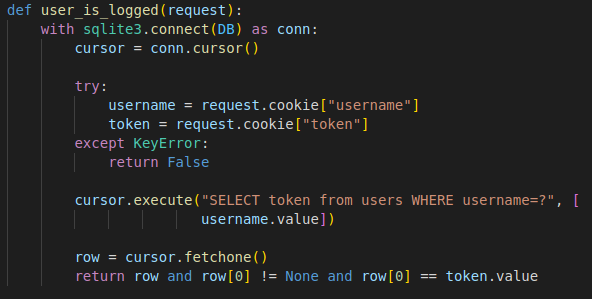
\includegraphics[height=4cm, width=8cm]{images/userislogged.png}
	\caption{Função user\_is\_logged}
	\label{fig.userislogged}
\end{figure} 

\subsection{Função db\_store\_image}
\label{ssec.funcaodbstoreimage}

Função utilizada para armazenar as imagens e os seus respetivos dados à \ac{bd} e criar uma nova coleção caso esta não exista.

\begin{figure}[H]
	\centering
	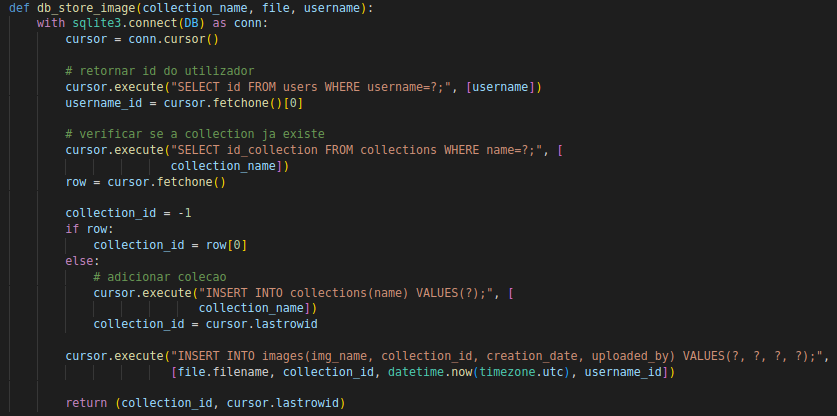
\includegraphics[height=4cm, width=8cm]{images/dbstoreimage.png}
	\caption{Função db\_store\_image}
	\label{fig.funcaodbstoreimage}
\end{figure} 

\subsection{Funções get}
\label{ssec.funcoesget}
Todas as funções \textit{get} presentes no programa \textit{web.py} são utilizadas para obter informações específicas relativas ao utilizador, às imagens e às coleções armazenadas na \ac{bd} \textit{cromos.db}.

\begin{figure}[H]%
    \centering
    \subfloat[\centering]{{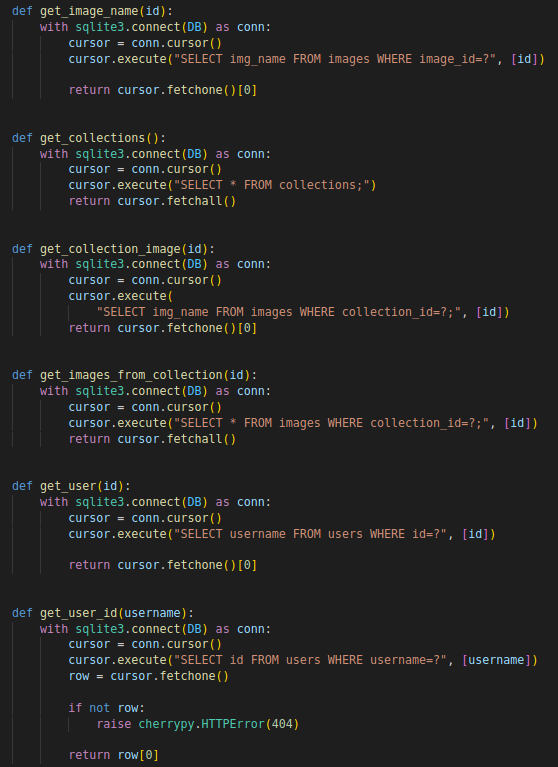
\includegraphics[height=7cm, width=5cm]{images/get1.png} }}%
    \qquad
    \subfloat[\centering]{{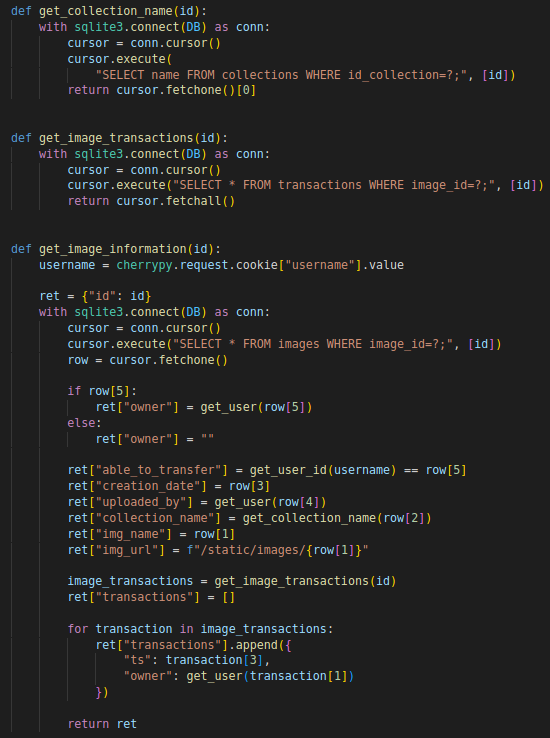
\includegraphics[height=7cm, width=5cm]{images/get2.png} }}%
    \caption{Funções get}%
    \label{fig:funcoesget}%
\end{figure}

\subsection{Função draft\_image}
\label{ssec.funcaodraftimage}

Sempre que um utilizador requisitar uma imagem, esta função será invocada com o propósito de atualizar as informações da imagem, na \ac{bd}, de acordo com os dados do novo proprietário.
Numa tabela chamada \textbf{transactions}, são inseridas informações os sobre a transação da imagem, ou seja, o \textit{id} do utilizador, a data de transação e o \textit{id} da imagem em questão. 

\begin{figure}[H]
	\centering
	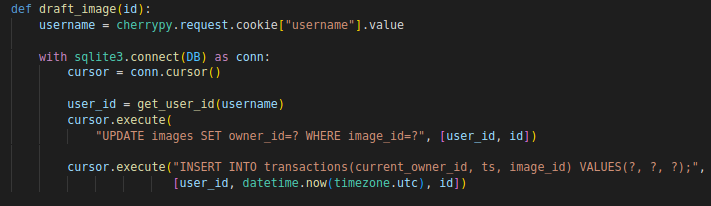
\includegraphics[height=3cm, width=12cm]{images/draftimage.png}
	\caption{Função draft\_image}
	\label{fig.funcaodbstoreimage}
\end{figure} 

\subsection{Função db\_update\_image\_owner}
\label{ssec.funcaodbupdateimageowner}

Numa situação em que o utilizador pretenda fazer uma troca de imagens com outro utilizador, esta função será invocada e irá atualizar, as informações, relativas à imagem, presentes na \ac{bd}, na tabela \textit{images}, de forma a atribuir um novo \textit{owner}. Quanto à tabela \textit{transactions}, esta será atualizada com as informações mais relevantes relativas à troca, tais como a data, o seu \textit{owner} atual e anterior e o \textit{id}.

\begin{figure}[H]
	\centering
	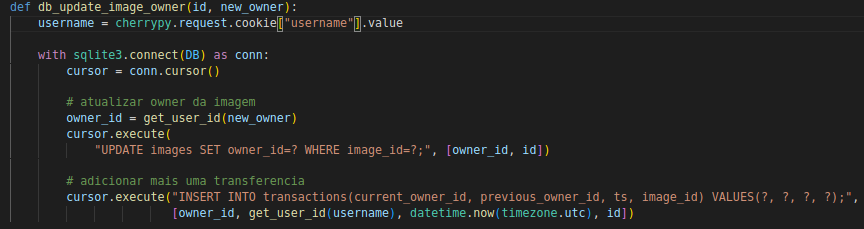
\includegraphics[height=3cm, width=12cm]{images/updateimageowner.png}
	\caption{Função db\_update\_image\_owner}
	\label{fig.funcaodbupdateimageowner}
\end{figure} 

\subsection{Classe CreateImage}
\label{ssec.classecreateimage}

A classe \textbf{CreateImage} é utilizada para o funcionamento do \textit{upload} de uma imagem, obtendo o nome da imagem e o seu ficheiro que serão utilizados na função \textbf{db\_store\_image} de modo a armazenar esta nova imagem.

\begin{figure}[H]
	\centering
	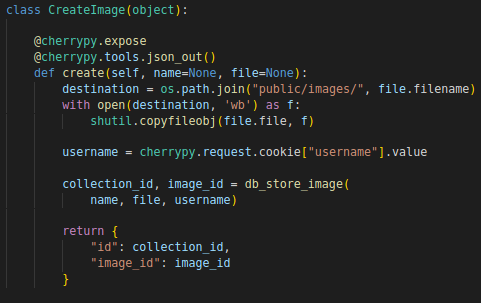
\includegraphics[height=6cm, width=12cm]{images/classecreateimage.png}
	\caption{Classe CreateImage}
	\label{fig.classecreateimage}
\end{figure} 

\subsection{Classe Users}
\label{ssec.users}

Dentro da classe \textbf{Users}, podemos encontrar funções relacionadas com a autenticação, criação e gestão de utilizadores.

Na função \textbf{auth}, após o \textit{login} por parte do utilizador, os seus dados vão ser comparados com os dados presentes na \ac{bd} (\textbf{cromos.db}) e, caso correspondam, é-lhe atribuído um \textit{token}. Este \textit{token} é gerado aleatóriamente e é composto por 8 caracteres \ac{ascii}.

A função \textbf{create} é utilizada para registar os dados do utilizador na \ac{bd} e a função \textbf{valid} retorna as \textit{strings} "valid" ou "invalid" dependendo se o utilizador está ou não conectado.

Por fim, a função \textbf{profile} é utilizada de forma a atualizar o perfil do utilizador com as imagens que este requisitou.

\begin{figure}[H]%
    \centering
    \subfloat[\centering]{{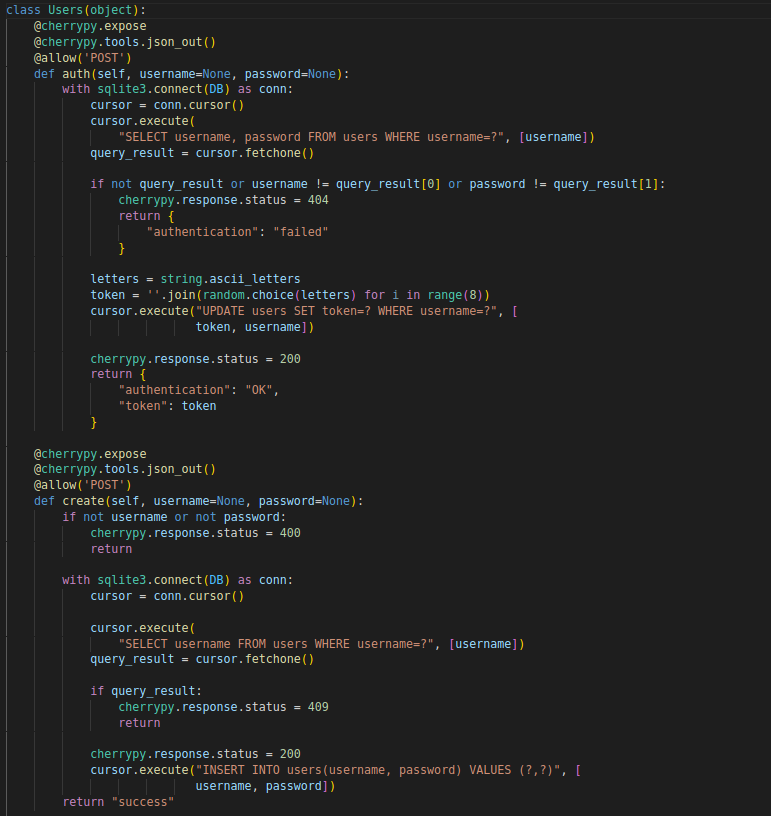
\includegraphics[height=7cm, width=7cm]{images/users1.png} }}%
    \qquad
    \subfloat[\centering]{{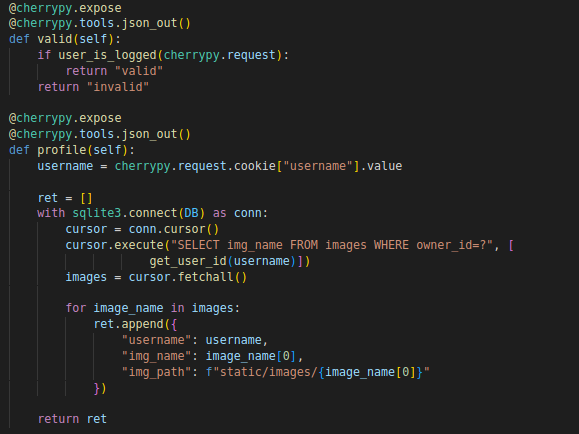
\includegraphics[height=4.5cm, width=7cm]{images/users2.png} }}%
    \caption{Classe Users}%
    \label{fig:usersimg}%
\end{figure}

\subsection{Classe Cromos}
\label{ssec.classecromos}

A classe \textbf{Cromos} é constituída pelas funções \textbf{index}, \textbf{draft}, \textbf{image} e \textbf{transfer}. Na primeira, caso não seja atribuído nenhum \textit{id}, a sua funcionalidade é armazenar todas as informações das imagens e das respetivas coleções num dicionário \ac{json} que será enviado para o \textit{front-end}; no caso de ser atribuído um \textit{id}, os efeitos serão os mesmos, mas para uma imagem específica. Na segunda, são invocadas as funções \textbf{draft\_image} e \textbf{watermark}, mencionadas anteriormente, que servirão para auxiliar o processo de requisição. A terceira serve o propósito de obter as informações completas de uma imagem associada a um \textit{id}. Por último, a função \textbf{transfer}, invoca as funções \textbf{db\_update\_image\_owner} e \textbf{watermark}, para serem utilizadas no processo de troca de imagem entre utilizadores.

\begin{figure}[H]%
    \centering
    \subfloat[\centering]{{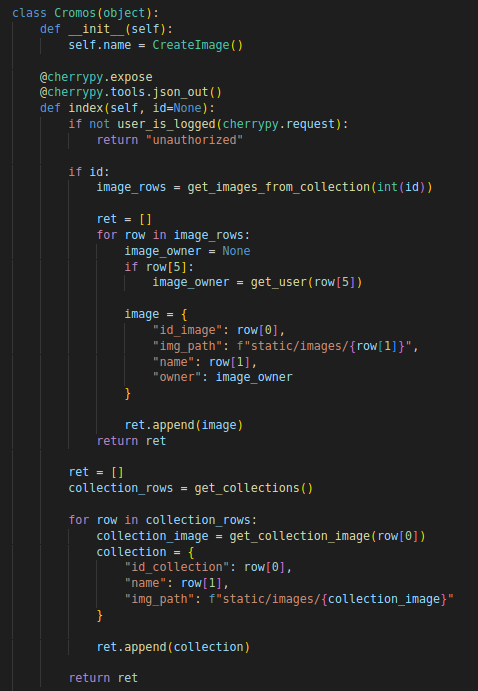
\includegraphics[height=7cm, width=7cm]{images/classecromos1.png} }}%
    \qquad
    \subfloat[\centering]{{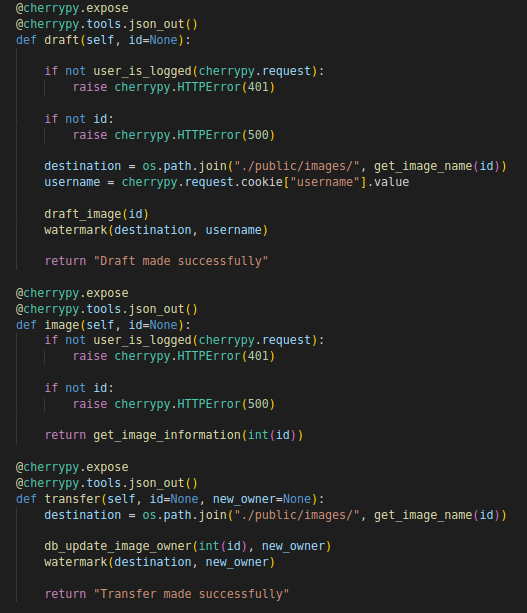
\includegraphics[height=7cm, width=7cm]{images/classecromos2.png} }}%
    \caption{Classe Cromos}%
    \label{fig:classecromos}%
\end{figure}

\subsection{Classe Root}
\label{ssec.root}

A função \textbf{\_\_init\_\_} classe \textbf{Root} permite a comunicação direta entre o \textit{back-end} e o \textit{front-end} utilizando dicionários \ac{json}.

As restantes funções utilizadas na \textbf{Root} servem para retornar o conteúdo \ac{html}.

\begin{figure}[H]%
    \centering
    \subfloat[\centering]{{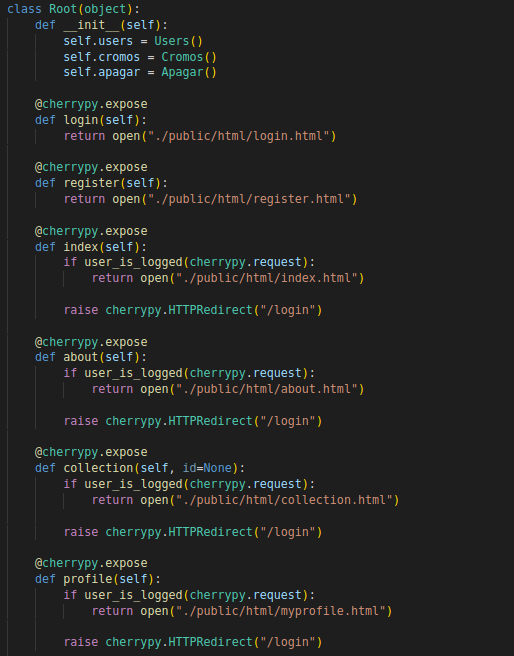
\includegraphics[height=6.5cm, width=5.5cm]{images/root1.png} }}%
    \qquad
    \subfloat[\centering]{{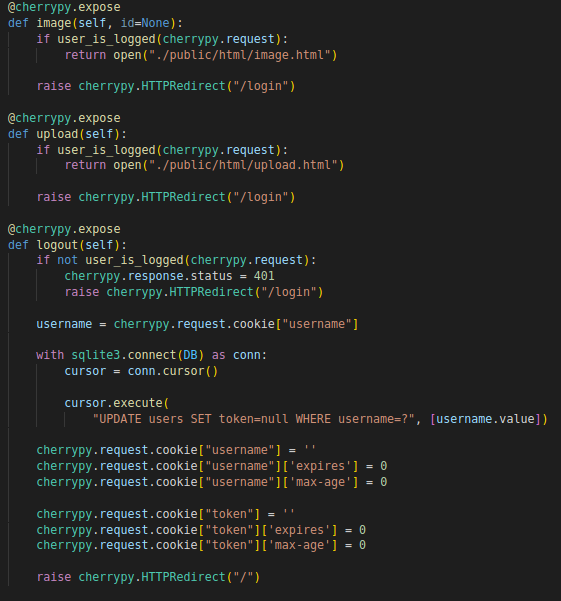
\includegraphics[height=6.5cm, width=5.5cm]{images/root2.png} }}%
    \caption{Classe Root}%
    \label{fig:rootimg}%
\end{figure}

\section{Persistência}
\label{sec.persistencia}

A \ac{bd} é composta por 4 tabelas relacionais, sendo estas denominadas por \textit{users}, \textit{images}, \textit{collections} e \textit{transactions}. Nas tabelas \textit{images}, \textit{transactions} e \textit{collections}, são feitas referências às chaves da tabela \textit{users} e, desta forma, é possível fazer a ligação entre as tabelas através do \textit{id} dos utilizadores e do \textit{id} da coleção.

\begin{figure}[H]%
    \centering
    \subfloat[\centering]{{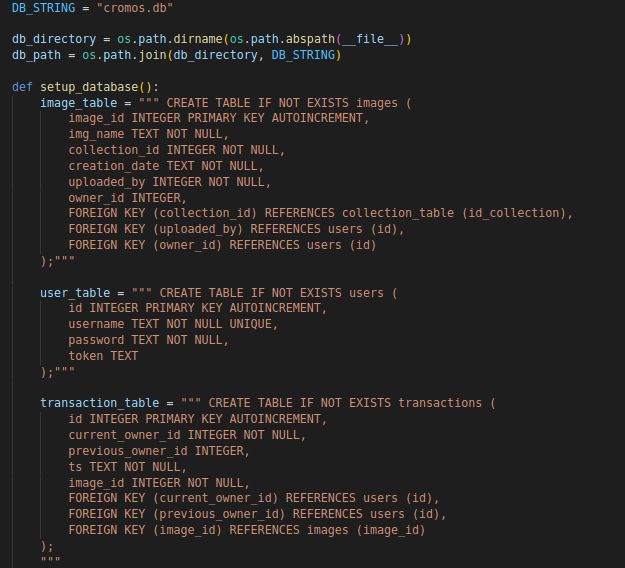
\includegraphics[height=5.5cm, width=5.5cm]{images/database1.png} }}%
    \qquad
    \subfloat[\centering]{{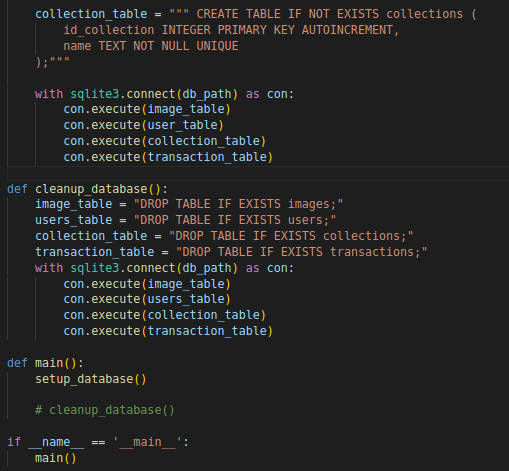
\includegraphics[height=5.5cm, width=5.5cm]{images/database2.png} }}%
    \caption{database.py}%
    \label{fig:databaseimg}%
\end{figure}

\section{Processador de Imagens}
\label{sec.procimagem}

Quanto ao processamento de imagem, este vai ser feito através da função \textbf{watermark}, presente no programa \textit{web.py}. Esta função é responsável por colocar uma marca de água, composta pelo \textit{username} do utilizador que fez a requisição, na imagem requisitada, de forma a poder identificar o seu atual proprietário. Esta imagem vai ser guardada no directório \textit{images}. 

\begin{figure}[H]
	\centering
	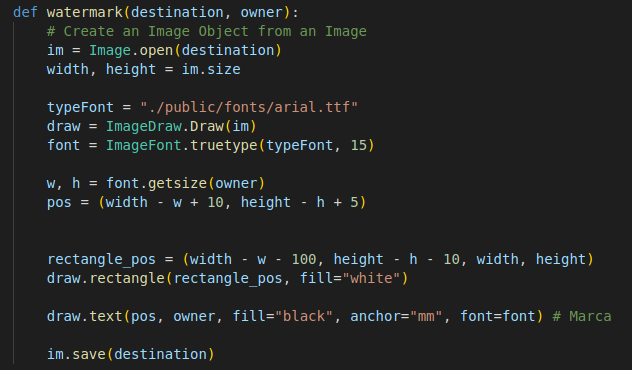
\includegraphics[height=4.5cm, width=7cm]{images/funcaowatermark.png}
	\caption{Função watermark}
	\label{fig.funcaowatermark}
\end{figure}

\chapter{Resultados}
\label{chap.resultados}

\begin{figure}[H]
    \centering
    \subfloat[\centering]{{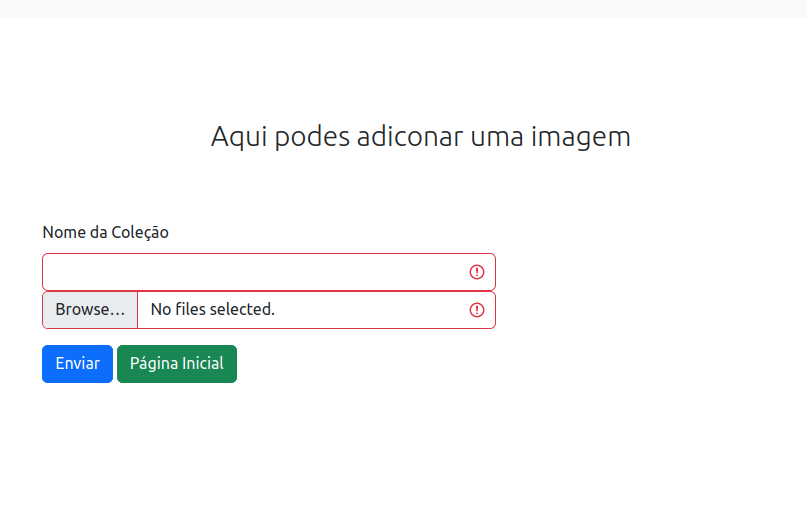
\includegraphics[height=6cm, width=5cm]{images/resultados3.png} }}
    \qquad
    \subfloat[\centering]{{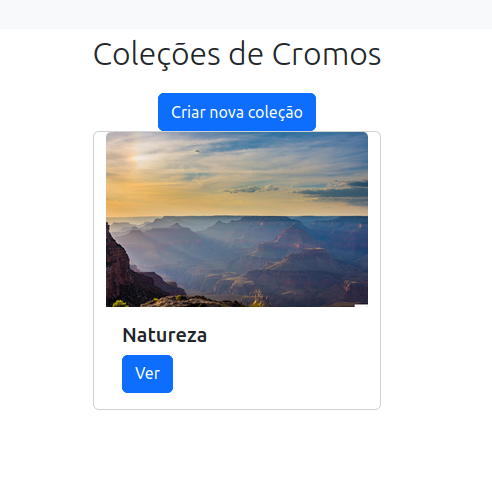
\includegraphics[height=5.5cm, width=5.5cm]{images/resultados1.png} }}
    \caption{É possível criar uma coleção atribuindo um nome à mesma e adicionando uma imagem (a); É possível ver todas as imagens disponíveis na coleção (b)}
    \label{fig:resultados1}
\end{figure}

\begin{figure}[H]
    \centering
    \subfloat[\centering]{{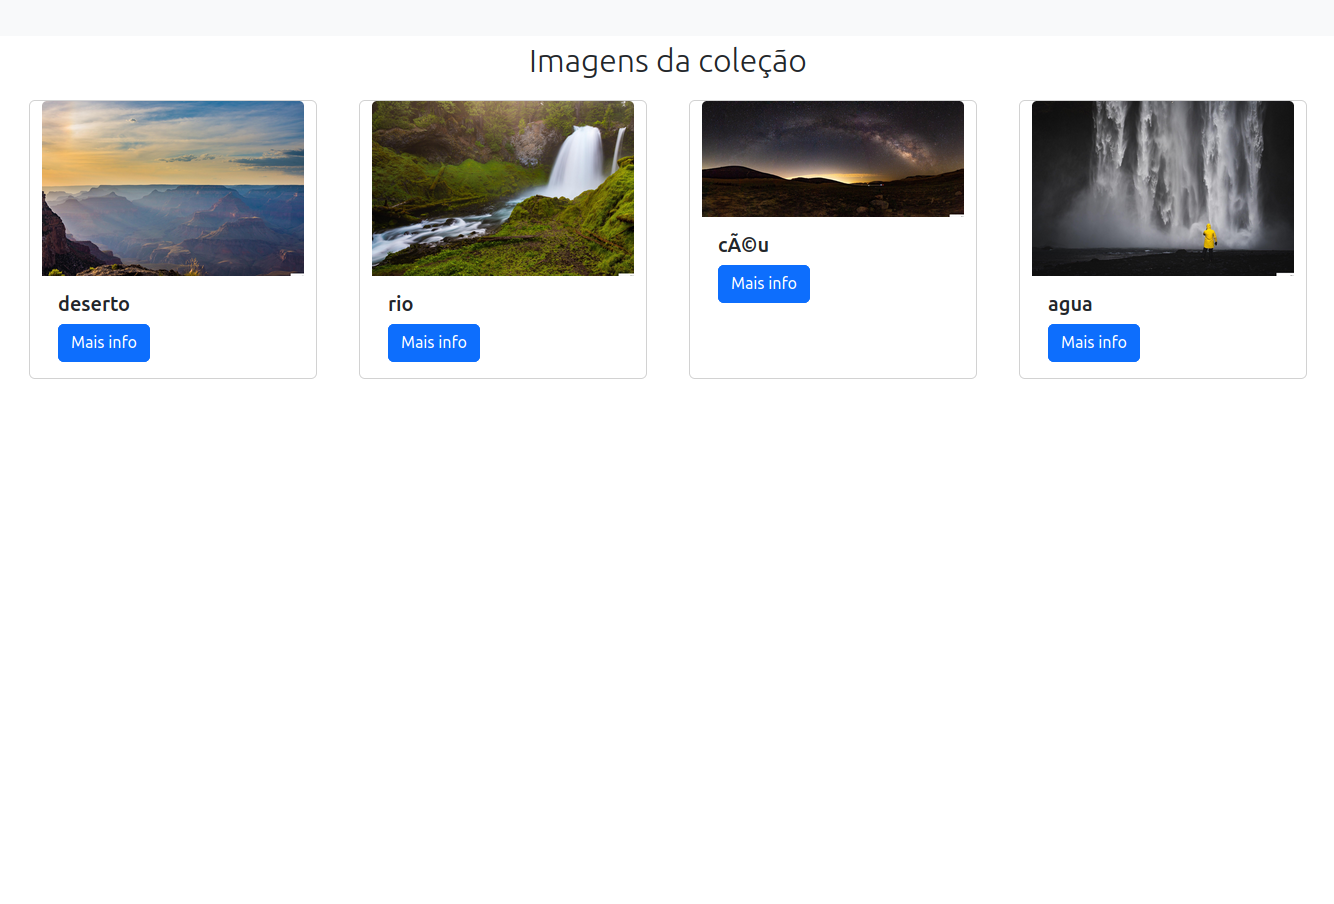
\includegraphics[height=5.5cm, width=5.5cm]{images/resultados2.png} }}
    \qquad
    \subfloat[\centering]{{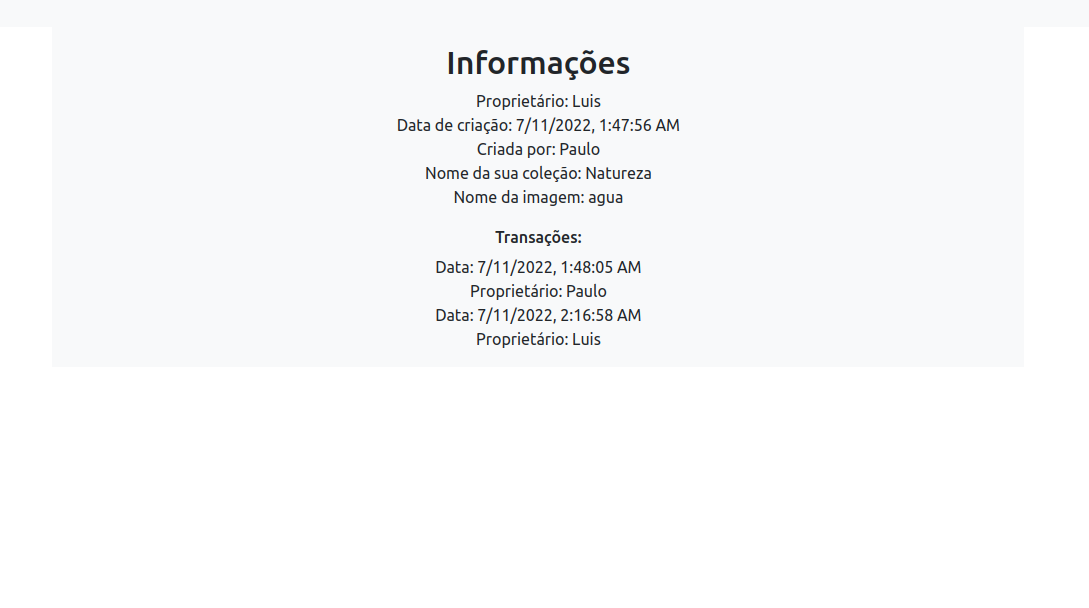
\includegraphics[height=5cm, width=5cm]{images/resultados4.png} }}
    \caption{São apresentadas todas as imagens da coleção (a) com a opção de ver as informações (b)}
    \label{fig:resultados2}
\end{figure}

\begin{figure}[H]
    \centering
    \subfloat[\centering]{{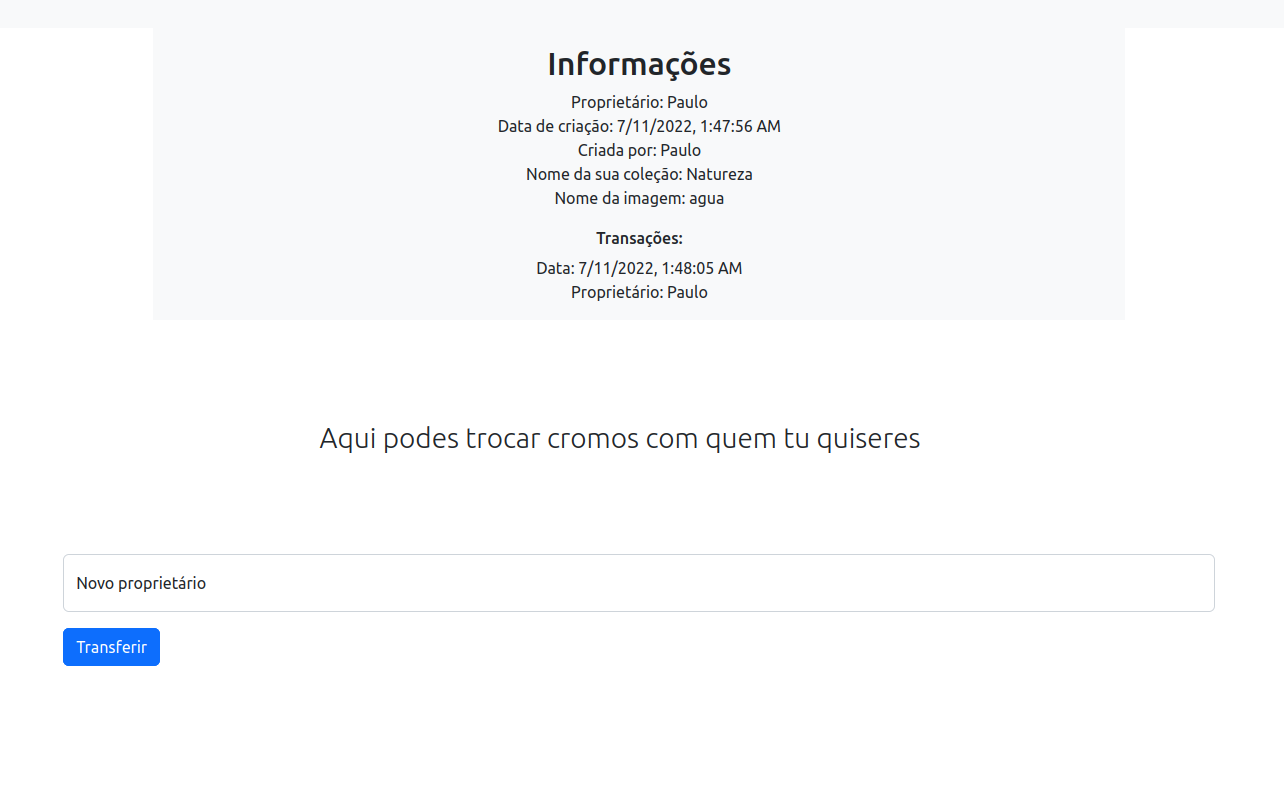
\includegraphics[height=5.5cm, width=5.5cm]{images/resultados5.png} }}
    \qquad
    \subfloat[\centering]{{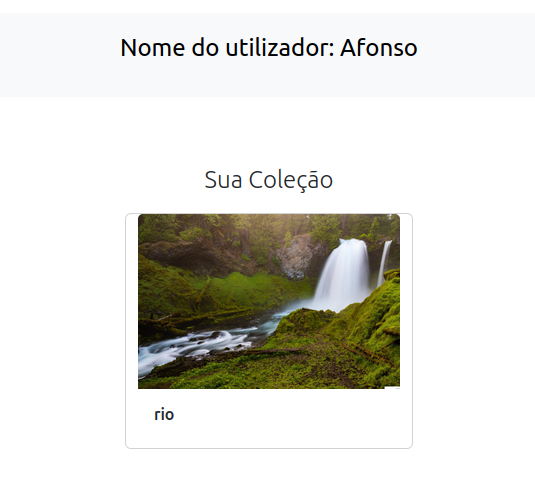
\includegraphics[height=5.5cm, width=5.5cm]{images/resultados6.png} }}%
    \caption{Também é possível transferir a imagem, caso seja o dono da mesma (a); Perfil do utilizador onde é apresentado o nome e a sua coleção pessoal (b)}
    \label{fig:resultados3}
\end{figure}

\chapter{Conclusões}
\label{chap.conclusao}
Graças a este projeto, foi possível adquirir e consolidar conhecimentos fundamentais para o desenvolvimento de aplicações web. 

É importante referir a utilização de \ac{js}, \ac{html}, \ac{css} e Bootstrap para o desenvolvimento do \textit{front-end} e Python, \ac{json}, jQuery, Ajax e SQLite, utilizados para desenvolver o \textit{back-end}. Estas "ferramentas" foram fundamentais para o projeto e são excelentes recursos para utilizar em trabalhos futuros.
 

\chapter*{Contribuições dos autores}

O \ac{ab} contribuiu para o \textit{web.py} , \ac{js} e ficou responsável pelo \textit{debugging}.
O \ac{ll} contribuiu para o \textit{web.py}, \textit{database.py}, \ac{css} e para o relatório.
O \ac{pm} contribui para o \textit{web.py}, \textit{database.py}, \ac{html}, \ac{js} e \ac{css}.

\vspace{10pt}

\autores : 30\%, 20\%, 50\%\\

%%%%%%%%%%%%%%%%%%%%%%%%%%%%%%%%%
\chapter*{Acrónimos}
\begin{acronym}
\acro{ua}[UA]{Universidade de Aveiro}
\acro{miect}[MIECT]{Mestrado Integrado em Engenharia de Computadores e Telemática}
\acro{lei}[LEI]{Licenciatura em Engenharia Informática}
\acro{uc}[UC]{Unidade Curricular}
\acro{labi}[LabI]{Laboratórios de Informática}
\acro{ab}[AB]{Afonso Baixo}
\acro{ll}[LL]{Luís Leal}
\acro{pm}[PM]{Paulo Macedo}
\acro{js}[JS]{JavaScript}
\acro{json}[JSON]{JavaScript Object Notation}
\acro{html}[HTML]{Hypertext Markup Language}
\acro{css}[CSS]{Cascading Style Sheets}
\acro{ascii}[ASCII]{American Standard Code for Information Interchange}
\acro{bd}[BD]{Base de Dados}
\end{acronym}


%%%%%%%%%%%%%%%%%%%%%%%%%%%%%%%%%
\bibliographystyle{plain}
\bibliography{bibliografia}

\end{document}
